\documentclass{article}[11pt]
\usepackage{fullpage,graphicx, setspace, latexsym, cite,amsmath,amssymb,xcolor,subfigure}
%\usepackage{epstopdf}
%\DeclareGraphicsExtensions{.pdf,.eps,.png,.jpg,.mps} 
\usepackage{amssymb} %maths
\usepackage{amsmath} %maths
\usepackage{amsthm, comment}
\usepackage[round,comma,sort,numbers]{natbib}

% \bibliographystyle{plain}
\bibliographystyle{plos2015}

\newtheorem{theorem}{Theorem}
\newtheorem{prop}{Proposition}
\newtheorem{corollary}{Corollary}
\newtheorem{lemma}{Lemma}
\newtheorem{defn}{Definition}
\newtheorem{ex}{Example}
\usepackage{float}

\newcommand*{\underuparrow}[1]{\underset{\uparrow}{#1}}
\usepackage{graphicx}
\usepackage{xcolor}
\usepackage[dvipsnames]{xcolor}
\usepackage{algorithmicx}
\usepackage{algorithm} %http://ctan.org/pkg/algorithms
\usepackage{algpseudocode} %http://ctan.org/pkg/algorithmicx
\usepackage{enumitem}
\usepackage{simplemargins}
\usepackage{hyperref}

\usepackage{mdframed}
\definecolor{lgray}{rgb}{0.92,0.92,0.92}
\definecolor{lsalmon}{rgb}{0.9921568627450981,0.9411764705882353, 0.9254901960784314}

\renewcommand{\bibnumfmt}[1]{#1.}
\setlist{noitemsep} % or \setlist{noitemsep} to leave space around whole list
\setallmargins{1in}
\linespread{1.1}

\newcommand{\brows}[1]{%
  \begin{bmatrix}
  \begin{array}{@{\protect\rotvert\;}c@{\;\protect\rotvert}}
  #1
  \end{array}
  \end{bmatrix}
}
\newcommand{\rotvert}{\rotatebox[origin=c]{90}{$\vert$}}
\newcommand{\rowsvdots}{\multicolumn{1}{@{}c@{}}{\vdots}}


\def\R{\mathbb{R}}
\def\Eps{\mathcal{E}}
\def\E{\mathbb{E}}
\def\V{\mathbb{V}}
\def\F{\mathcal{F}}
\def\G{\mathcal{G}}
\def\H{\mathcal{H}}
\def\S{\mathcal{S}}
\def\D{\mathcal{D}}
\def\P{\mathbb{P}}
\def\1{\mathbf{1}}
\def\n{\nappa}
\def\h{\mathbf{w}}
\def\v{\mathbf{v}}
\def\x{\mathbf{x}}
\def\X{\mathcal{X}}
\def\Y{\mathcal{Y}}
\def\eps{\epsilon}
\def\y{\mathbf{y}}
\def\e{\mathbf{e}}
\newcommand{\norm}[1]{\left|\left|#1\right|\right|}
\DeclareMathOperator*{\argmin}{arg\,min}
\DeclareMathOperator*{\argmax}{arg\,max}
\newcommand{\lecture}[4]{
   \pagestyle{myheadings}
   \thispagestyle{plain}
   \newpage
   % \setcounter{lecnum}{#1}
   \setcounter{page}{1}
   \setlength{\headsep}{10mm}
   \noindent
   \begin{center}
   \framebox{
      \vbox{\vspace{2mm}
    \hbox to 6.28in { {\bf CHEME 5820: Machine Learning for Engineers
   \hfill Spring 2025} }
       \vspace{4mm}
       \hbox to 6.28in { {\Large \hfill Lecture #1: #2  \hfill} }
       \vspace{2mm}
       \hbox to 6.28in { {\it Lecturer: #3 \hfill #4} }
      \vspace{2mm}}
   }
   \end{center}
   \markboth{Lecture #1: #2}{Lecture #1: #2}

   \noindent{\bf Disclaimer}: {\it These notes have not been subjected to the
   usual scrutiny reserved for formal publications. }
   \vspace*{4mm}
}

\begin{document}
\lecture{3a}{Linear Regression, Perceptron and Binary Classification}{Jeffrey Varner}{}

\begin{mdframed}[backgroundcolor=lgray]
    In this lecture, we will discuss the following topics:
    \begin{itemize}[leftmargin=16pt]
        \item{\textbf{Supervised learning} is a type of machine learning where the model is trained on labeled data, meaning that each training example includes both the input features (measurements) and the corresponding target (output) variable. The goal is to learn a mapping from inputs to outputs so that the model can make accurate predictions on new, unseen data.}
        \item{\textbf{Linear regression} is a statistical method for modeling the relationship between a target variable (output) and one or more features (input) by fitting a linear model to observed data. It provides a simple way to predict outcomes and understand relationships between variables. The model is linear in the parameters, not necessarily in the features.}
        \item{\textbf{Continuous variable prediction tasks}: In machine learning, linear regression models are commonly employed for continuous variable prediction tasks. These models enable the estimation of numerical outcomes based on the (non)linear relationships identified between input features and the target variable.}
        \item{\textbf{Binary classification tasks}: While linear regression is primarily designed to predict continuous outcomes, it can also be adapted for classification tasks by combining the linear regression model with an output function that transforms the continuous target variable predictions into discrete classes or probability estimates. In this lecture, we'll consider binary classification using \href{https://en.wikipedia.org/wiki/Perceptron}{the perceptron classification algorithm developed at Cornell in the 1950s}.}
    \end{itemize}
 \end{mdframed}

\section{Introduction}
This lecture will introduce supervised learning and linear models for regression and classification tasks.
The supervised learning problem requires a dataset and a learning algorithm \href{https://github.com/kuleshov/cornell-cs5785-2024-applied-ml}{figured reproduced from the Applied Machine Learning (Cornell CS5785, Fall 2024) course}:
\begin{equation*}
\underbrace{\text{Dataset}}_\text{Features, Attributes, Targets} + \underbrace{\text{Learning Algorithm}}_\text{Model Class + Objective + Optimizer } \to \text{Predictive Model}
\end{equation*}
The output of the supervised learning problem is a predictive model that maps inputs to targets. 
Today, we'll examine linear models. These models are easy to implement and interpret and serve as a foundation for the more complex predictive models we'll explore.
In particular, we will discuss estimating the parameters of a linear model for overdetermined systems, and then we'll pivot to the classification problem. However, before getting to the linear models, we will first introduce the optimizer and gradient descent (a quick review of some items from the calculus course you took in high school or college).

\section{Optimizer}
The material in this section was heavily inspired by the \href{https://github.com/kuleshov/cornell-cs5785-2024-applied-ml}{Applied Machine Learning (Cornell CS5785, Fall 2024) course notes.} Before we present our first supervised learning algorithm, linear regression, let's do a quick calculus review related to the supervised learning problem. 

\subsection{Calcular Review}
A key part of a supervised learning algorithm is the \texttt{optimizer}, which takes  
an objective $J$ (also called a loss function) and a model $\mathcal{M}$ and tries to find the best model $f$ in $\mathcal{M}$ that minimizes the objective $J$. In general, an objective function $J$ measures the difference between the predicted values and the observed values in some way, e.g., the mean squared error (MSE), the cross-entropy loss, or the negative log-likelihood.
The optimizer outputs a model $f \in \mathcal{M}$ with the smallest value of the objective $J$, i.e., $\min_{f \in \mathcal{M}} J(f)$. Intuitively, this is the function that best describes the (training) dataset
$\mathcal{D} = \{(\mathbf{x}_{i}, y_{i}) \mid i = 1,2,\dots,n\}$. But what is this magical \texttt{optimizer} creature?
As it turns out, the \texttt{optimizer} can be many different things, but in this lecture, we will focus on the \texttt{gradient descent optimizer}. This approach uses the gradient of the objective function to find its minimum.

\subsubsection*{Gradient}
The key tool from calculus that we will use to develop the \texttt{gradient descent optimizer} is the derivative and its extensions. Suppose we have a univariate function $f_{\theta}: \mathbb{R} \to \mathbb{R}$. The derivative ${d f}/{d \theta}$ (evaluated at $\theta_0$) is the instantaneous rate of change of the function $f(\theta)$ with respect to its parameter $\theta$ at the point $\theta_0$. The partial derivative ${\partial f(\theta)}/{\partial \theta_j}$ of a multivariate function $f : \mathbb{R}^d \to \mathbb{R}$ is the derivative of $f$ with respect to $\theta_j$ 
while all the other dimensions $\theta_k$ for $k\neq j$ are held constant. Finally, the gradient $\nabla_{\theta} f$ of the multivariate function $f$ with respect to the vector $\theta$ is the vector of all the partial derivatives:
\begin{equation}
\nabla_{\theta} f (\theta) = \begin{bmatrix}
\frac{\partial f(\theta)}{\partial \theta_1} \\
\frac{\partial f(\theta)}{\partial \theta_2} \\
\vdots \\
\frac{\partial f(\theta)}{\partial \theta_d}
\end{bmatrix}
\end{equation}
The $j$th entry of the gradient is the partial derivative ${\partial f}/{\partial \theta_j}$ of $f$ with respect to the $j$th component of $\theta$. We are interested in the gradient because it tells us the direction of the steepest ascent of the function $f$ at the point $\theta_0$. We also know that when the gradient is zero, i.e., $\nabla_{\theta} f(\theta_0) = \mathbf{0}$, then we have a local minimum or maximum of the function $f$.

\subsubsection*{Gradient descent}
Suppose there exists an objective function $J(\theta)$ that we want to minimize with respect to the parameters $\theta$. 
Gradient descent is a numerical search algorithm that minimizes an objective function by iteratively adjusting the parameters in the opposite direction of the gradient:
\begin{equation*}
    \theta_{k+1} = \theta_{k} - \alpha(k)\cdot\nabla{J}(\theta_{k})\quad\text{where}{~k = 0,1,2,\dots}
\end{equation*}
where $k$ denotes the iteration index, and $\alpha(k)>0$ is a hyperparameter called the learning rate, which can be a function of the iteration count $k$.
We iterate until a stopping criterion is met, i.e., $\norm{\theta_{k+1} - \theta_{k}}\leq\epsilon$, the maximum number of iterations is reached, or some other stopping criterion is met.
A pseudocode for a naive gradient descent algorithm (for a fixed learning rate) is shown in Algorithm \ref{alg:gd}.
\begin{algorithm}[H]
\caption{Naive Gradient Descent for objective ${J}(\theta)$}\label{alg:gd}
\begin{algorithmic}[1]
\State \textbf{Input:} Initial parameters $\theta_0$, learning rate $\alpha$, stopping criterion $\epsilon$, maximum iterations $N$
\State \textbf{Output:} Optimal parameter estimates $\theta$
\State Initialize $\theta \gets \theta_0$\Comment{Initialize parameters to the initial guess}
\State $k \gets 0$\Comment{Initialize iteration counter}
\While{$k \leq N$ \textbf{or} $\|\theta_{k+1}  - \theta_{k} \| \leq \epsilon$}
    \State $\mathbf{d} \gets \nabla J(\theta_{k})$\Comment{Compute gradient using analytical or numerical method, evaluate at $\theta_{k}$}
    \State $\theta_{k+1} \gets \theta_{k} - \alpha \cdot \mathbf{d}$\Comment{Update parameters using the gradient direction $\mathbf{d}$}
    \State $k \gets k + 1$
\EndWhile

\State \textbf{return} $\theta$
\end{algorithmic}
\end{algorithm}

\section{Linear Models}
Linear models are a class of models used in machine learning for regression tasks, i.e., predicting a continuous output variable from one or more continuous or discrete input features.
Linear models assume that the output variable is a linear combination of the input features, i.e., a linear function of the input features weighted by some parameters.
Linear in this context is a misnomer because the features are not necessarily linear, but the model is linear in terms of the parameters and features.
Suppose we have a data set $\mathcal{D} = \left\{(\mathbf{x}_{i},y_{i}) \mid i=1,2,\dots,n\right\}$ with $n$ examples, where each example where $\mathbf{x}_{i}\in\R^{m}$ is a feature vector and $y_{i}\in\R$ is the output variable.
The linear regression model predicts the output variable $y_{i}$ for feature vector $\hat{\mathbf{x}}_{i}$ using the linear function:
\begin{equation*}
    y_{i} = \hat{\mathbf{x}}_{i}^{\top}\beta + \epsilon_{i}
\end{equation*}
where we have augmented the feature vector with a bias term, i.e., $\hat{\mathbf{x}}_{i}^{\top} = \left(x^{(i)}_{1},\dots,x^{(i)}_{m},1\right)$, $\beta\in\mathbb{R}^{p}$ is a $p=m+1$ dimensional column vector of (unknown) parameters to be estimated, and $\epsilon_{i}\sim\mathcal{N}(0,\sigma^{2})$ is a noise term, typically assumed to be a Normal distribution with mean zero and variance $\sigma^{2}$.
Depending upon the shape of the data and various other problem constraints, 
there may be an \textit{analytical solution} for the linear model parameter vector $\beta$, e.g., the normal equations, or we can estimate an iterative solution using an optimizer such as gradient descent.
Let's first consider the analytical solution for the linear regression parameter vector $\beta$ for an \textit{overdetermined} system of equations.

\subsection{Overdetemined linear models with regularization}
If the number of examples $n$ is greater than the number of features $m$, the linear model is said to be \texttt{overdetermined}.
In other words, there are more examples than features.  Regularized linear regression models incorporate penalty terms to constrain the size of the coefficient estimates, 
thereby reducing overfitting and enhancing the model's generalizability to new data. 
Consider an overdetermined data matrix $\hat{\mathbf{X}}\in\mathbb{R}^{n\times{p}}$, i.e., the case where $n\gg{p}$ (there are many more examples than unknown parameters)
whose rows are the augmented feature vectors:
\begin{equation*}
\hat{\mathbf{X}} = 
    \brows{\hat{\mathbf{x}}_1^\top \\ \hat{\mathbf{x}}_2^\top \\ \rowsvdots \\ \hat{\mathbf{x}}_n^\top}
\end{equation*}
A regularized least squares estimate of the expected value of the unknown model parameters $\hat{\mathbf{\beta}}$ for an overdetermined system will minimize a loss (objective) function of the form:
\begin{equation}\label{eq:regressionloss-regularization-L2}
\hat{\mathbf{\beta}}_{\lambda} = \arg\min_{\mathbf{\beta}} \frac{1}{2}\norm{\mathbf{y} - \hat{\mathbf{X}}\mathbf{\beta}}^{2}_{2} + 
\frac{\lambda}{2}\norm{\mathbf{\beta}}^{2}_{2}
\end{equation}
where $||\star||^{2}_{2}$ is the square of the $L2$-vector norm (Euclidean norm), the parameter
$\lambda\geq{0}$ denotes a regularization parameter (user-defined hyperparameter), 
and $\hat{\mathbf{\beta}}_{\lambda}$ denotes the estimated expected parameter vector. 
The expected value of the parameters $\hat{\mathbf{\beta}}_{\lambda}$ that minimize the $||\star||^{2}_{2}$ loss plus penalty for the overdetermined data matrix $\mathbf{X}$ is given by:
\begin{equation*}
\hat{\mathbf{\beta}}_{\lambda} = \left(\hat{\mathbf{X}}^{\top}\hat{\mathbf{X}}+\lambda\cdot\mathbf{I}\right)^{-1}\hat{\mathbf{X}}^{\top}\mathbf{y}
\end{equation*}
where $\mathbf{I}$ is the identity matrix.
The matrix $\hat{\mathbf{X}}^{\top}\hat{\mathbf{X}}+\lambda\cdot\mathbf{I}$ is the $\texttt{regularized normal matrix}$, while $\hat{\mathbf{X}}^{\top}\mathbf{y}$ is the $\texttt{moment vector}$. 
The inverse $\left(\hat{\mathbf{X}}^{\top}\hat{\mathbf{X}}+\lambda\cdot\mathbf{I}\right)^{-1}$ must exist to obtain the estimated parameter vector $\hat{\mathbf{\beta}}_{\lambda}$.
If we estimate (or propose) an error model, we can then compute the \textit{uncertainty} of the estimated parameter vector $\hat{\mathbf{\beta}}_{\lambda}$ as:
\begin{equation*}
\hat{\mathbf{\beta}}^{\dagger}_{\lambda} = \hat{\mathbf{\beta}}_{\lambda} - \left(\hat{\mathbf{X}}^{\top}\hat{\mathbf{X}}+\lambda\cdot\mathbf{I}\right)^{-1}\hat{\mathbf{X}}^{\top}\mathbf{\epsilon}
\end{equation*}
Let's look at the overdetermined linear regression solution without regularization and how the solution is obtained.
The steps below can also be applied to the regularized case (but we'll skip the details).

\subsubsection*{Derivation: Overdetermined solution without regularization}
To better understand the overdetermined linear regression solution, let's consider a simple example without regularization, i.e., $\lambda=0$. The objective function described in Eq. \ref{eq:regressionloss-regularization-L2} can be rewritten form as:
\begin{equation}\label{eq:regressionloss-regularization-L2-2}
J(\beta) = \frac{1}{2}(\hat{\mathbf{X}} \beta - \mathbf{y})^\top  (\hat{\mathbf{X}} \beta - \mathbf{y})
\end{equation}
We can compute the gradient of the mean squared error as:
\begin{align*}
\nabla_\beta J(\beta) 
& = \nabla_\beta \frac{1}{2} (X \beta - y)^\top  (\hat{\mathbf{X}} \beta - \mathbf{y}) \\
& = \frac{1}{2} \nabla_\beta \left( (\hat{\mathbf{X}} \beta)^\top  (\hat{\mathbf{X}} \beta) - (\hat{\mathbf{X}} \beta)^\top \mathbf{y} - \mathbf{y}^\top (\hat{\mathbf{X}} \beta) + \mathbf{y}^\top \mathbf{y} \right) \\
& = \frac{1}{2} \nabla_\beta \left( \beta^\top  (\hat{\mathbf{X}}^\top \hat{\mathbf{X}}) \beta - 2(\hat{\mathbf{X}} \beta)^\top \mathbf{y} \right) \\
& = \frac{1}{2} \left( 2(\hat{\mathbf{X}}^\top \hat{\mathbf{X}}) \beta - 2X^\top \mathbf{y} \right) \\
& = (\hat{\mathbf{X}}^\top \hat{\mathbf{X}}) \beta - \hat{\mathbf{X}}^\top \mathbf{y}
\end{align*}
We used the facts that $a^\top b = b^\top a$ (line 3), that $\nabla_x b^\top \hat{\mathbf{X}} = b$ (line 4), and that $\nabla_x x^\top A x = 2 A x$ for a symmetric matrix $A$ (line 4).
Setting the gradient to zero, we get the \texttt{normal equations}, which we can solve for the unknown parameters $\beta$:
\begin{align*}
(\hat{\mathbf{X}}^\top \hat{\mathbf{X}}) \beta - \hat{\mathbf{X}}^\top \mathbf{y} 
& = 0 \\
(\hat{\mathbf{X}}^\top \hat{\mathbf{X}}) \beta 
& = \hat{\mathbf{X}}^\top \mathbf{y} \\
\hat{\beta} 
& = (\hat{\mathbf{X}}^\top \hat{\mathbf{X}})^{-1} \hat{\mathbf{X}}^\top \mathbf{y}
\end{align*}
The uncertainty of the estimated parameter vector $\hat{\mathbf{\beta}}$ can be computed as (assuming we have an error model with mean zero):
\begin{align*}
   \mathbf{y} 
   & = \hat{\mathbf{X}}\cdot\hat{\mathbf{\beta}} + \mathbf{\epsilon} \\
   \hat{\mathbf{X}}^{\top}\mathbf{y}
   & = \hat{\mathbf{X}}^{\top}\hat{\mathbf{X}}\mathbf{\beta} + \hat{\mathbf{X}}^{\top}\mathbf{\epsilon} \\
   \hat{\mathbf{X}}^{\top}\hat{\mathbf{X}}\mathbf{\beta} 
    & = \hat{\mathbf{X}}^{\top}\mathbf{y} - \hat{\mathbf{X}}^{\top}\mathbf{\epsilon} \\
    \hat{\mathbf{\beta}}^{\dagger} 
    & = \left(\hat{\mathbf{X}}^{\top}\hat{\mathbf{X}}\right)^{-1}\hat{\mathbf{X}}^{\top}\mathbf{y} - \left(\hat{\mathbf{X}}^{\top}\hat{\mathbf{X}}\right)^{-1}\hat{\mathbf{X}}^{\top}\mathbf{\epsilon}
\end{align*}
which is the same as:
\begin{align*}
   \hat{\mathbf{\beta}}^{\dagger} 
    & = \hat{\mathbf{\beta}} - \left(\hat{\mathbf{X}}^{\top}\hat{\mathbf{X}}\right)^{-1}\hat{\mathbf{X}}^{\top}\mathbf{\epsilon}
\end{align*}

\subsubsection*{Error Models}
In the previous section, we assumed the error model was a Normal distribution with mean zero and variance $\sigma^{2}$. 
This is a common assumption in linear regression, but it may not always be true. Therefore, it is a good idea to examine the residuals. The residuals are the difference between the observed values and the predicted values, i.e., $\mathbf{r} = \mathbf{y} - \hat{\mathbf{X}}\hat{\mathbf{\beta}}$. 
If the error model is correct, the residuals should be normally distributed with mean zero and constant variance. 
We can use a variety of statistical tests to check the normality of the residuals, e.g., 
the \href{https://en.wikipedia.org/wiki/Shapiro–Wilk_test}{Shapiro-Wilk test}, the \href{https://en.wikipedia.org/wiki/Kolmogorov–Smirnov_test}{Kolmogorov-Smirnov test}, 
or the \href{https://en.wikipedia.org/wiki/Anderson–Darling_test}{Anderson-Darling test}.
We can estimate the parameters of the error using \href{https://en.wikipedia.org/wiki/Maximum_likelihood_estimation}{maximum likelihood estimation} (MLE).
We'll talk more about MLE and an alternative approach called \href{https://en.wikipedia.org/wiki/Maximum_a_posteriori_estimation}{maximum a posteriori estimation} in a future lecture.
So, for now, let's move on to the classification problem.

\begin{figure}
    \centering
	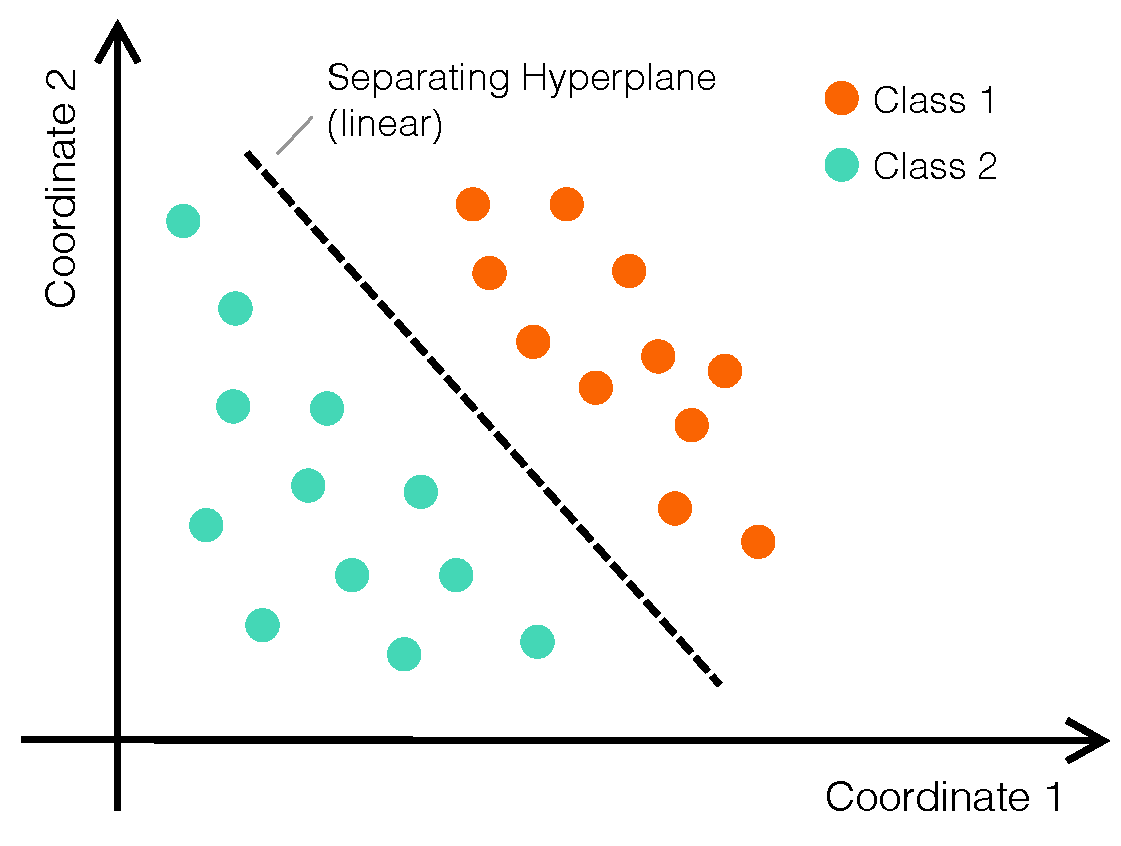
\includegraphics[width=0.5\textwidth]{./figs/Fig-LinearSeperableData-Hyperplane.pdf}
	\caption{Schematic of a binary classification task with linearly separable data.
    Above the hyperplane are positive examples, while below the hyperplane are negative examples.}\label{fig:linearhyperplane}
\end{figure}

\section{The Perceptron and Binary Classification}
The Perceptron \cite{Perceptron1960} is a simple yet powerful algorithm used in machine learning for binary classification tasks.
\href{https://en.wikipedia.org/wiki/Perceptron}{The Perceptron (Rosenblatt, 1957)} takes the (scalar) output of a linear regression model $y_{i}\in\mathbb{R}$ and then transforms 
it using the $\sigma(\star) = \texttt{sign}(\star)$ function to a discrete set of values representing categories, e.g., $\sigma:\mathbb{R}\rightarrow\{-1,1\}$ in the binary classification case. 

Suppose there exists a data set
$\mathcal{D} = \left\{(\mathbf{x}_{1},y_{1}),\dotsc,(\mathbf{x}_{n},y_{n})\right\}$ with $n$ labeled examples, where each example has been labeled by an expert, i.e., a human to be in a category $\hat{y}_{i}\in\{-1,1\}$, given the $m$-dimensional feature vector $\mathbf{x}_{i}\in\mathbb{R}^{m}$.  
\href{https://en.wikipedia.org/wiki/Perceptron}{The Perceptron} \textit{incrementally learns} a linear decision boundary between two classes of possible objects (binary classification) in $\mathcal{D}$ by repeatedly processing the data. 
During each pass, a regression parameter vector $\mathbf{\beta}$ is updated until it makes no more than a specified number of mistakes. 
\href{https://en.wikipedia.org/wiki/Perceptron}{The Perceptron} computes the estimated label $\hat{y}_{i}$ for feature vector $\hat{\mathbf{x}}_{i}$ using the $\texttt{sign}:\mathbb{R}\to\{-1,1\}$ function:
\begin{equation*}
    \hat{y}_{i} = \texttt{sign}\left(\hat{\mathbf{x}}_{i}^{\top}\cdot\beta\right)
\end{equation*}
where $\beta=\left(w_{1},\dots,w_{n}, b\right)$ is a column vector of (unknown) classifier parameters, 
$w_{j}\in\mathbb{R}$ corresponding to the importance of feature $j$ and $b\in\mathbb{R}$ is a bias parameter, 
the features $\hat{\mathbf{x}}^{\top}_{i}=\left(x^{(i)}_{1},\dots,x^{(i)}_{m}, 1\right)$ are $p = m+1$-dimensional (row) vectors 
(features augmented with bias term), and $\texttt{sign}(z)$ is the function:
\begin{equation*}
    \texttt{sign}(z) = 
    \begin{cases}
        1 & \text{if}~z\geq{0}\\
        -1 & \text{if}~z<0
    \end{cases}
\end{equation*}
If data set $\mathcal{D}$ is linearly separable, the Perceptron will incrementally learn a separating hyperplane in a finite number of passes through the $\mathcal{D}$. 
However, if the data set $\mathcal{D}$ is not linearly separable, the Perceptron may not converge. 
A pseudocode for the perceptron algorithm is shown in Algorithm~\ref{alg:perceptron}.
\begin{algorithm}[H]
    \caption{The Perceptron Algorithm}\label{alg:perceptron}
    \begin{algorithmic}[1]
        % \Procedure{Incremental-Training-Perceptron}{$\mathcal{D}$}
        \State \textbf{Input:} $\mathcal{D} = \left\{(\mathbf{x}_{1},y_{1}),\dotsc,(\mathbf{x}_{n},y_{n})\right\}$, tolerance $\epsilon\geq{0}$, maximum iterations $\texttt{maxiter}$
        \State \textbf{Features:} $\hat{\mathbf{x}}_{i} = \left(x_{i1},\dots, x_{im},1\right)$ are augmented with a bias term, labels $y_{i}\in\{-1,1\}$.
        \State \textbf{Output:} Classifier parameters $\mathbf{\beta} = \left(w_{1},\dots, w_{m}, b\right)$
        \State $\mathbf{\beta} \gets \texttt{rand}$\Comment{Initialize parameter vector $\mathbf{\beta}$ to a random vector}
        \State $i \gets 0$\Comment{Initialize the loop counter to zero}
        \While{$\text{true}$}\Comment{Repeat until stopping criterion is met}
        \State $\text{error} \gets 0$\Comment{Initialize the error count to zero for this pass through $\mathcal{D}$}
        \For{$(\mathbf{x},y)\in\mathcal{D}$}\Comment{Iterate over each pair $(\mathbf{x},y)$ in data set $\mathcal{D}$}
            \If{$y\cdot\left(\mathbf{x}^{\top}\cdot\mathbf{\beta}\right) \leq 0$}\Comment{Ooops! The data pair $(\mathbf{x},y)$ is misclassified}
                \State $\mathbf{\beta} \gets \mathbf{\beta} + {y}\cdot\mathbf{x}$\Comment{Update the weight vector $\mathbf{\beta}$}
                \State $\text{error} \gets \text{error} + 1$\Comment{Increment the error count}
            \EndIf
        \EndFor
        \If{$\text{error} \leq \epsilon$ \textbf{or} $i\geq\texttt{maxiter}$ }\Comment{Stopping criterion: tolerance or max iterations?}
            \State \textbf{break} \Comment{Exit the training loop}    
        \EndIf
        \State $i \gets i + 1$\Comment{Increment the loop counter and repeat}
        \EndWhile
        % \EndProcedure
    \end{algorithmic}
\end{algorithm}
What the algorithm does is to update the weight vector $\mathbf{\beta}$ for each example $(\mathbf{x}_{i},y_{i})$ in the data set $\mathcal{D}$.
If the example is misclassified, i.e., $y_{i}\left(\mathbf{x}_{i}^{\top}\cdot\mathbf{\beta}\right)\leq{0}$, the weight vector $\mathbf{\beta}$ is updated by adding the feature vector $\mathbf{x}_{i}$ multiplied by the label $y_{i}$.
The algorithm continues to iterate through the data set $\mathcal{D}$ until all examples are correctly classified or until a stopping criterion is met, e.g., a maximum number of iterations or a tolerance on the number of classification errors.
In the end, the alogrithm estimates a linear hyperplane $\mathcal{H} = \left\{\mathbf{x}~|~\mathbf{x}^{\top}\cdot\mathbf{\beta} = 0\right\}$ that separates the two classes of data points in $\mathcal{D}$ (Fig. \ref{fig:linearhyperplane}).
The perceptron algorithm is guaranteed to converge to a solution if the data set is linearly separable in a finite number of passes through the data set.
For a proof of this convergence guarantee, see \href{https://www.cs.cornell.edu/courses/cs4780/2018fa/lectures/lecturenote03.html}{the CS4780 lecture notes from 2018}.

\section{Evaluation of the Binary Classifier}
Once the Perceptron (or any binary classifier) has converged, we can evaluate the binary classifier's performance using various metrics.
See Sidey-Gibbon et al. \cite{SG2019} for a detailed discussion of these metrics in the context of medical classification problems.
The central idea is to compare the predicted labels $\hat{y}_{i}$ to the actual labels $y_{i}$ in the data set $\mathcal{D}$. 
Various metrics can be used to evaluate the performance of a binary classifier, but they all start with computing the confusion matrix.

\begin{figure}
    \centering
	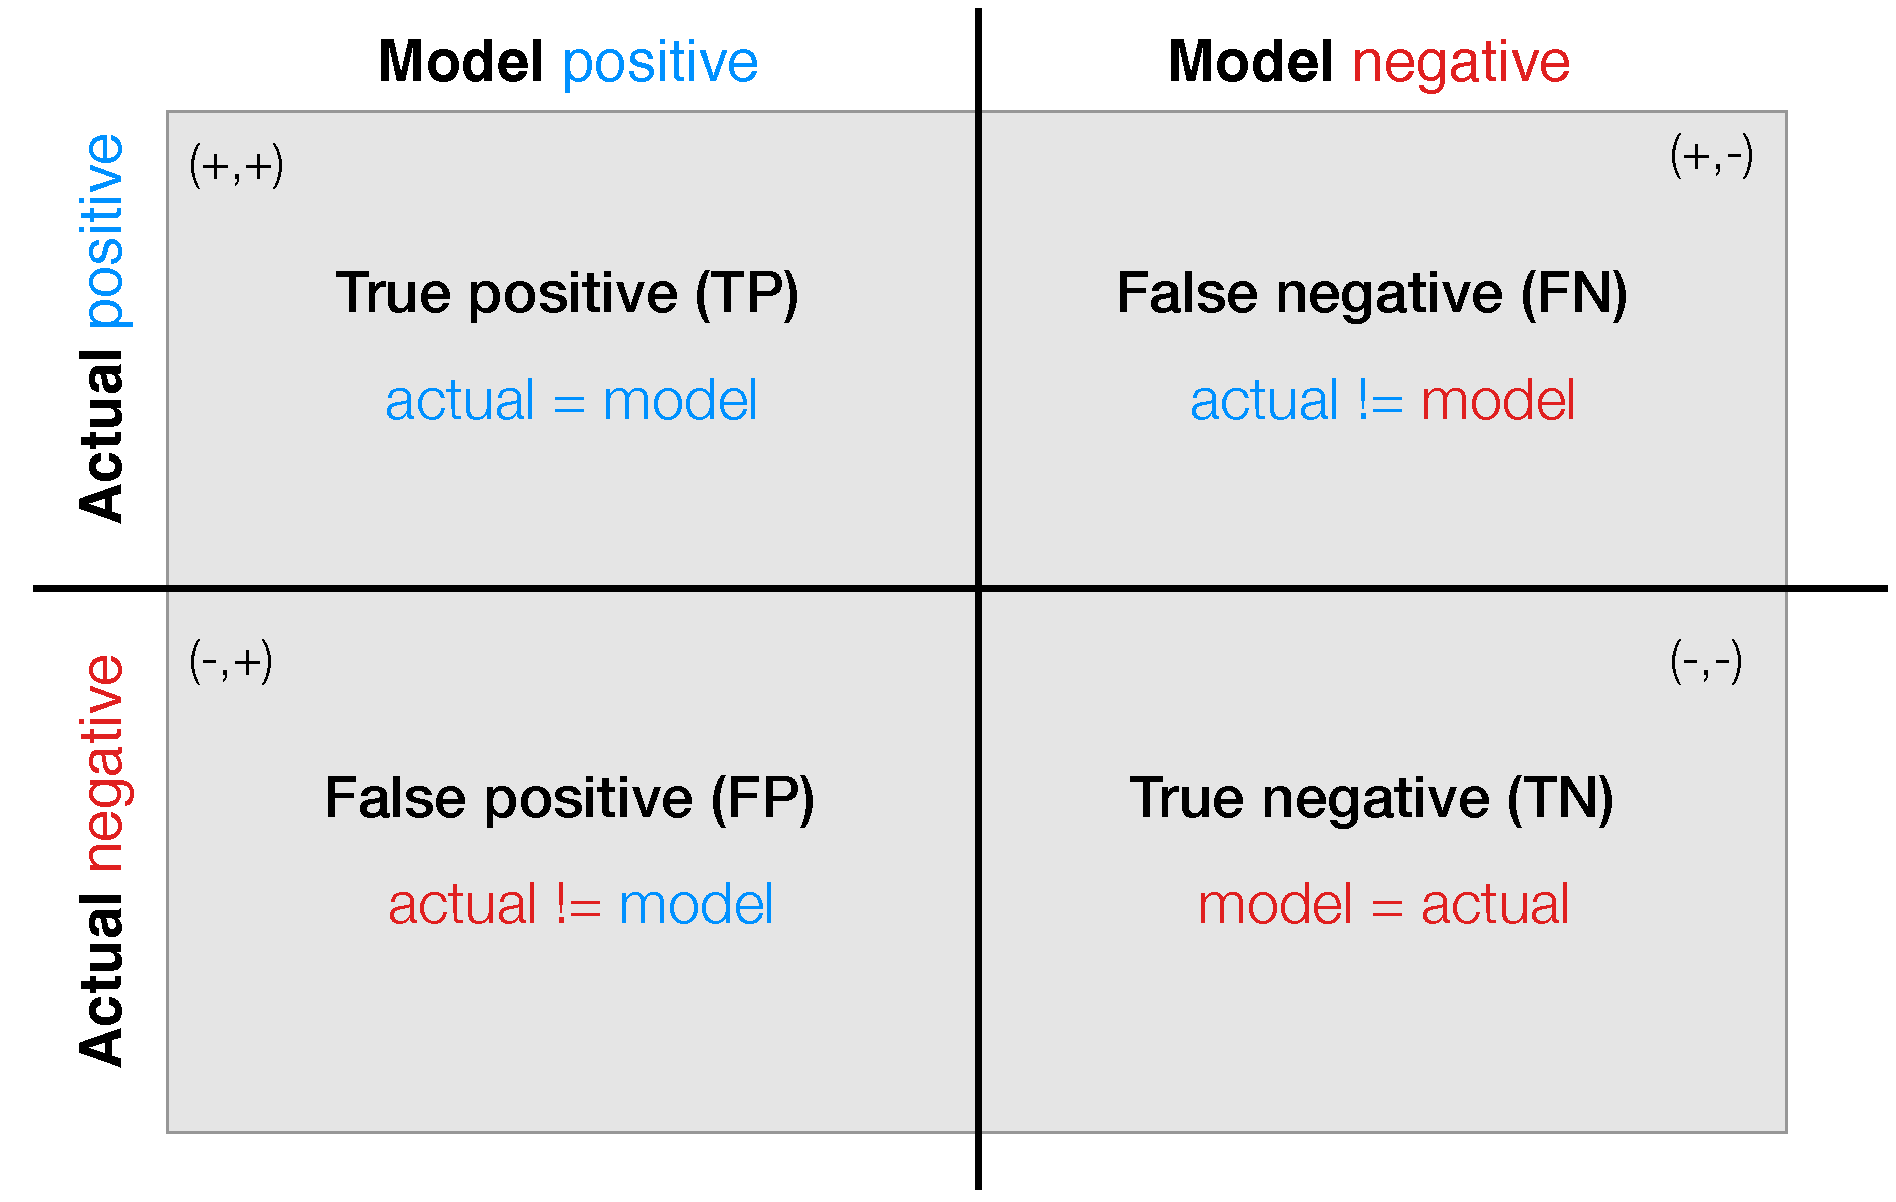
\includegraphics[width=0.75\textwidth]{./figs/Fig-BinaryConfusionMatrix.pdf}
	\caption{Confusion matrix schematic for the binary classification problem.}\label{fig:binaryconfusionmatrx}
\end{figure}

\subsection{Confusion Matrix}
The confusion matrix is a table often used to describe the performance of a classification model on a set of data for which the true values are known (Fig. \ref{fig:binaryconfusionmatrx}).
The confusion matrix is a $2\times{2}$ matrix that contains four entries: true positive (TP), false positive (FP), true negative (TN), and false negative (FN).
The true positive (TP) entry in the confusion matrix is the number of positive examples that were correctly classified as positive.
The false negative (FN) entry is the number of positive examples that were incorrectly classified as negative by the model.
The false positive (FP) entry is the number of negative examples that were incorrectly classified as positive by the model.
The true negative (TN) entry is the number of negative examples that were correctly classified as negative by the model.
The confusion matrix is used to calculate a variety of performance metrics, including accuracy, precision, recall, and the F1 score.

\paragraph*{Accuracy.}
The accuracy of a binary classifier is the proportion of correctly classified \textit{total} examples in the data set.
The accuracy is calculated as the sum of the true positive and true negative entries in the confusion matrix divided by the total number of examples in the data set:
\begin{equation}
    \text{Accuracy} = \frac{TP + TN}{TP + TN + FP + FN}
\end{equation}
Thus, accuracy measures the classifier's overall performance and indicates how well it can correctly classify examples (both positive and negative).

\paragraph*{Precision.}
The precision of a binary classifier is the proportion of correctly classified \textit{positive} examples out of all examples that were classified as positive by the model.
The precision is calculated as the true positive entry in the confusion matrix divided by the sum of the true positive and false positive entries:
\begin{equation}
    \text{Precision} = \frac{TP}{TP + FP}
\end{equation}
Precision measures the classifier's ability to classify positive examples correctly, and it is useful when the cost of false positives is high.

\paragraph*{Recall (Sensitivity).}
The recall of a binary classifier is the proportion of correctly classified \textit{positive} examples out of all truly positive examples in the data set.
The recall is calculated as the true positive entry in the confusion matrix divided by the sum of the true positive and false negative entries:
\begin{equation}
    \text{Recall} = \frac{TP}{TP + FN}
\end{equation}
Recall measures the classifier's ability to correctly classify positive examples, and it is useful when the cost of false negatives is high.

\paragraph*{F1 Score.}
The F1 score of a binary classifier is the harmonic mean of precision and recall. The F1 score is calculated as:
\begin{equation}
    \text{F1 Score} = 2\cdot\frac{\text{Precision}\cdot\text{Recall}}{\text{Precision} + \text{Recall}}
\end{equation}
The F1 score measures the classifier's overall performance and balances the trade-off between precision and recall.

\section{Summary}
This lecture introduced supervised learning and linear models for regression and classification tasks.
We discussed overdetermined linear models with regularization and the derivation of the analytical solution for the linear regression parameter vector $\beta$.
We also introduced a model to compute the uncertainty of the estimated parameter vector $\hat{\mathbf{\beta}}$.
Finally, we introduced the perceptron algorithm for binary classification problems.
The perceptron is a simple linear classifier that can be used to separate two classes of data points.
The perceptron algorithm is an iterative algorithm that incrementally updates the weights of the linear classifier to minimize the classification error.
Thus, it is one of the first examples of an online learning algorithm, i.e., an algorithm that learns from data incrementally.
The perceptron algorithm can converge to a solution if the data set is linearly separable.
However, if the data set is not linearly separable, the perceptron algorithm will not converge to a perfect solution (i.e., zero classification error).
Suppose we are willing to accept some classification errors. In that case, we can use the perceptron algorithm to find a separating hyperplane in a finite number of passes through the data set, 
even if the data set is not linearly separable, where some examples are misclassified.

\bibliography{References-L3a.bib}

\end{document}